
\subsection{Existierende Entitäten}
Die Menge an derzeit existierenden Entitäten in einem \textit{Core ECS} Programm ist definiert über

\[
    \text{live}(c) \coloneqq \bigcup_{i \in I} \text{dom}(c_i)
\]

\noindent
und entspricht also der Menge an Entitätstermen, die eine Assoziation zu einem Komponententerm enthalten.

\bigskip
\begin{tcolorbox}[excursusbox,title={Menge der gültigen Entitäten in SparseSet-Implementierungen}]
    $\text{live}(c)$ lässt sich auf eine übliche \textit{SparseSet}-Implementierung übertragen.
    Wenn ein \textit{SparseSet} Terme $k_i \in K_i$ verwaltet, dann enthält $\text{live}(c)$ alle $e_m$, die über die Sparse-Arrays verteilt als Index auf einen Komponententerm im Dense-Array verweisen (siehe Abbildung~\ref{fig:live_domain}).

    \[
        \begin{alignat}{3}
        \text{Sparse}_i &: E \rightharpoonup \mathcal{D}_i \\
        \text{Dense}_i &: \mathcal{D}_i \rightarrow K_i, \mathcal{D}_i \subseteq \mathbb{N}_0
        \end{alignat}
    \]
    \noindent
    und damit alternativ zu der im Text vorgestellten Notation
    \[
        c_i = \text{Dense}_i \circ \text{Sparse}_i
    \]
    

    \begin{center}
        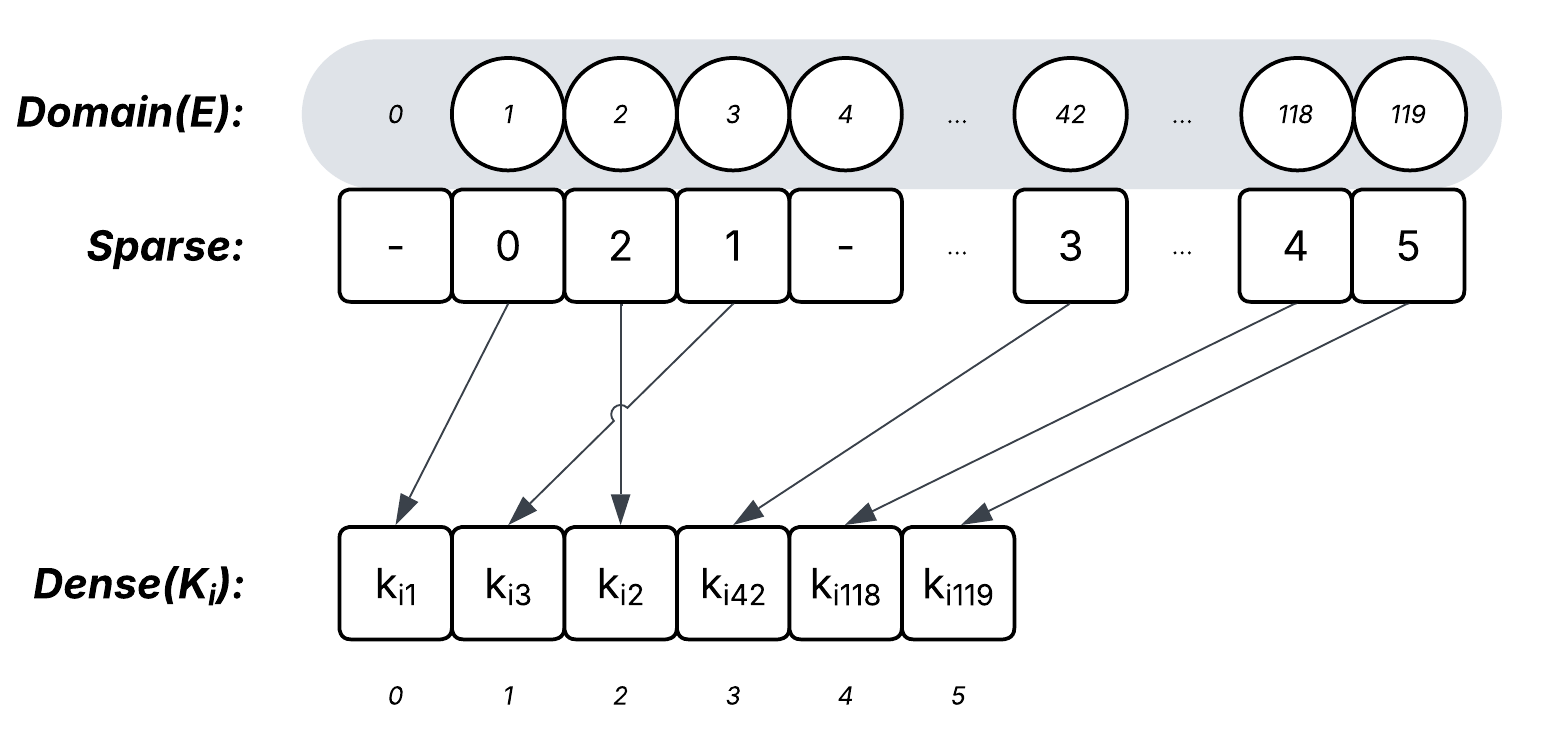
\includegraphics[width=0.8\columnwidth]{content/de/appendix/concurrency_paper/notation/img/sparse_set_domain}
        \captionof{figure}{Illustration einer Überführung der Notation als \textit{Sparse Set}-Implementierung. Der Definitionsbereich \textit{Domain(E)} ist hier an kein Label $i \in I$ gebunden, weil ein $e_m \in E$ als \textit{sparse index} über die \textit{Sparse Sets} mehrfach auftreten kann (siehe Abbildung~\ref{fig:sparse_sets}).  (Quelle: eigene Darstellung)}
        \label{fig:live_domain}
    \end{center}

    \begin{center}
        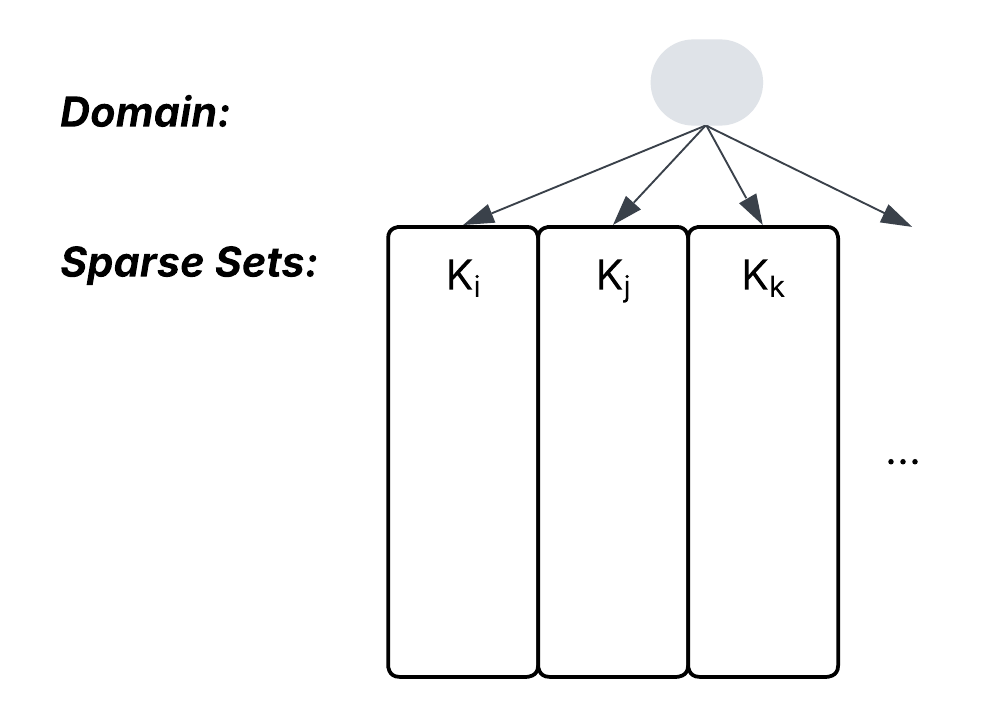
\includegraphics[width=0.5\columnwidth]{content/de/appendix/concurrency_paper/notation/img/sparse_sets}
        \captionof{figure}{Verteilung des Wertebereiches $\text{Domain}(E)$ über mehrere \textit{Sparse Sets}.  (Quelle: eigene Darstellung)}
        \label{fig:sparse_sets}
    \end{center}

\end{tcolorbox}
